% CVPR 2022 Paper Template
% based on the CVPR template provided by Ming-Ming Cheng (https://github.com/MCG-NKU/CVPR_Template)
% modified and extended by Stefan Roth (stefan.roth@NOSPAMtu-darmstadt.de)

\documentclass[10pt,twocolumn,letterpaper]{article}

%%%%%%%%% PAPER TYPE  - PLEASE UPDATE FOR FINAL VERSION
%\usepackage[review]{cvpr}      % To produce the REVIEW version
\usepackage{cvpr}              % To produce the CAMERA-READY version
%\usepackage[pagenumbers]{cvpr} % To force page numbers, e.g. for an arXiv version

% Include other packages here, before hyperref.
\usepackage{graphicx}
\usepackage{amsmath}
\usepackage{amssymb}
\usepackage{booktabs}


% It is strongly recommended to use hyperref, especially for the review version.
% hyperref with option pagebackref eases the reviewers' job.
% Please disable hyperref *only* if you encounter grave issues, e.g. with the
% file validation for the camera-ready version.
%
% If you comment hyperref and then uncomment it, you should delete
% ReviewTempalte.aux before re-running LaTeX.
% (Or just hit 'q' on the first LaTeX run, let it finish, and you
%  should be clear).
\usepackage[pagebackref,breaklinks,colorlinks]{hyperref}


% Support for easy cross-referencing
\usepackage[capitalize]{cleveref}
\crefname{section}{Sec.}{Secs.}
\Crefname{section}{Section}{Sections}
\Crefname{table}{Table}{Tables}
\crefname{table}{Tab.}{Tabs.}


%%%%%%%%% PAPER ID  - PLEASE UPDATE
\def\cvprPaperID{*****} % *** Enter the CVPR Paper ID here
\def\confName{CVPR}
\def\confYear{2022}


\begin{document}

%%%%%%%%% TITLE - PLEASE UPDATE
\title{Comparing Transformers and CNNs on the SpaceNet Flood Detection Challenge}

\author{Adrian Stoll\\
Stanford University\\
{\tt\small adrs@stanford.edu}
\and
Naijing Guo\\
Stanford University\\
{\tt\small njguo@stanford.edu}
\and
Nenad Bozinovic\\
Stanford University\\
{\tt\small nesa@stanford.edu}
}
\maketitle

%%%%%%%%% ABSTRACT

\begin{abstract}
    Our project compares transformer and CNN based semantic segmentation techniques on the SpaceNet flood detection challenge. The SpaceNet challenge is to segment buildings and roads from satellite photos taken before and after a flood and identify flooded roads segments and buildings. Winners of previous SpaceNet challenges and the baseline model for the most recent challenge use CNN backbone models. We hypothesize using transformer models for the backbone will improve segmentation performance by taking advantage of global characteristics of the image. We will test this hypothesis by training models with CNN and transformer backbones and comparing the results.
\end{abstract}

%%%%%%%%% BODY TEXT
\section{Introduction}
\label{sec:intro}

Floods are among the most devastating natural disasters, causing significant damage to buildings, infrastructure, and human life, as well as exacerbating environmental problems such as erosion and land degradation. Remote sensing, specifically satellite imagery analysis, has become a vital tool for flood detection and monitoring, providing fast initial mapping of flooded regions and helping in post-disaster assessments. 

The SpaceNet8 Challenge \cite{spacenet8} aims at developing open-source computer vision and machine learning methods for remote sensing data in the context of floods caused by hurricanes and heavy rains. The goal of this challenge is to rapidly develop maps and analyze the scale of destruction to better direct resources and first responders in real-world disaster scenarios by leveraging the existing repository of datasets and algorithms from SpaceNet Challenges 1-7 and expanding to multiclass feature extraction and characterization. We use the SpaceNet 8 dataset and focuses on infrastructure and flood mapping, addressing the extraction and characterization of building footprints and road networks. 

\section{Dataset}

We use SpaceNet8 dataset described in detail \href{https://openaccess.thecvf.com/content/CVPR2022W/EarthVision/papers/Hansch_SpaceNet_8_-_The_Detection_of_Flooded_Roads_and_Buildings_CVPRW_2022_paper.pdf}{here} \cite{spacenet8}. Data has been acquired using Maxar’s Earth observation satellites (data under creative common license). For SpaceNet8 dataset, two distinct areas of interest (AOIs) were selected that were flooded in 2021 (Germany and Louisiana). Data consists of pansharpened RGB (0.3-0.8m resolution) that are routinely published through Maxar Open Data Program.

Data was pre-labeled by analysts for both the pre- and post-event images. A road segment is considered flooded if it is visibly covered with water or rubble in the post-event imagery. If a building is assigned the flooded attribute, it means that there is flood water in its immediate proximity which is a proxy for probable flooding (since it is not possible from satellite imagery to determine whether a building is actually flooded inside). In the event that cloud cover obscured features in the post-event image, as is often the case in flooding disasters, analysts labeled only visible areas and not make any assumptions where features could not be seen (Figure \ref{fig:dataset1}).

Pre- and post-event images are not co-localized, i.e. do not overlap perfectly, and in fact might have different resolutions. The post-event
patches cover the same area on the ground but have different pixel sizes. Masks are build from GeoJSON data, where, for example, only vertices of the building polygon mask are stored, vs full mask image (more details \href{https://medium.com/the-downlinq/getting-started-with-spacenet-data-827fd2ec9f53}{here}).

\begin{figure}[t]
  \centering
   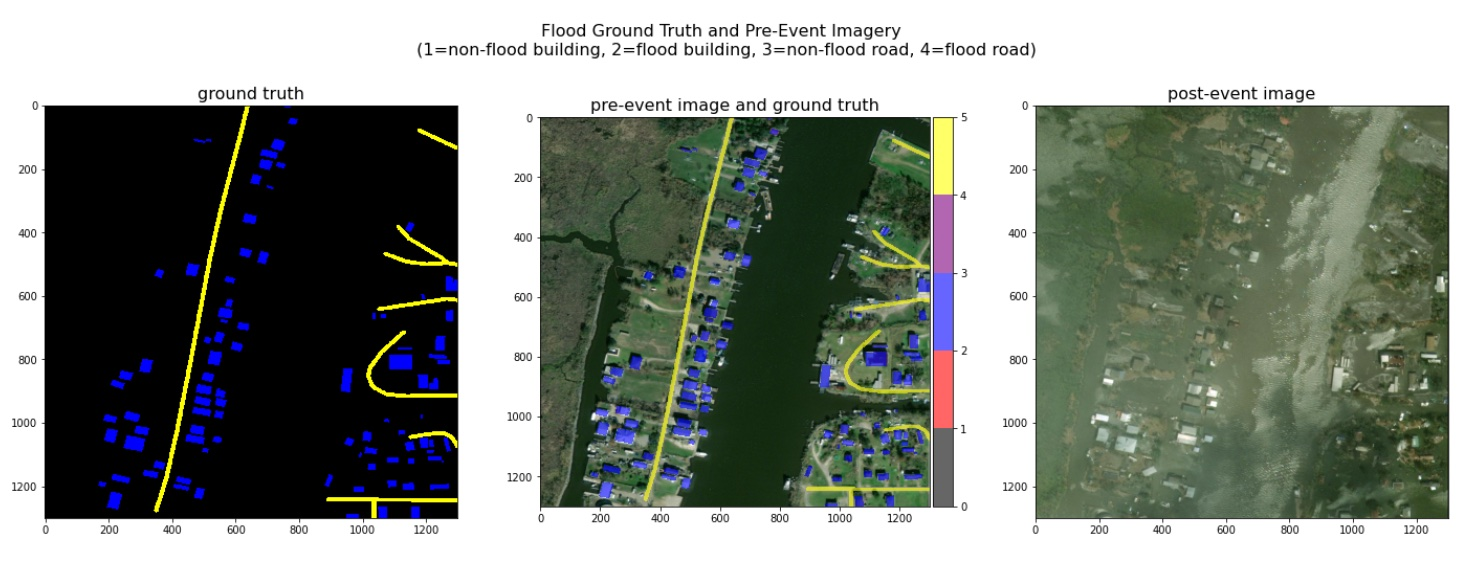
\includegraphics[width=1.0\linewidth]{figures/dataset1.jpg}
   \caption{Ground truth label (left), pre-event image (middle) and post-event image (right) of a flooded area. Flood labels
are created as four channel masks. Channel 1 corresponds
to non-flooded buildings, channel 2 for flooded buildings,
channel 3 for non-flooded roads, and channel 4 for flooded
roads. For example blue and yellow colors in the figure refer to flooded building and road.}
   \label{fig:dataset1}
\end{figure}

\section{Technical Approach}

\subsection{Baseline}

The proposed baseline (SpaceNet8 paper) consists of two independently trained convolutional neural networks: the Foundation network (responsible for
segmenting buildings and roads from the pre-event imagery
without any flood attribution), and the Flood network (responsible for predicting the flood status of roads and buildings by using both
pre- and post-event imagery as input). In addition to road detection, the foundation network includes road speed segmentation (i.e. 8 classes in increments of 10 mph). We will be focus on flooding aspect only for this project. Figure \ref{fig:baseline} gives an overview of main components of the baseline method.

\begin{figure}[t]
  \centering
   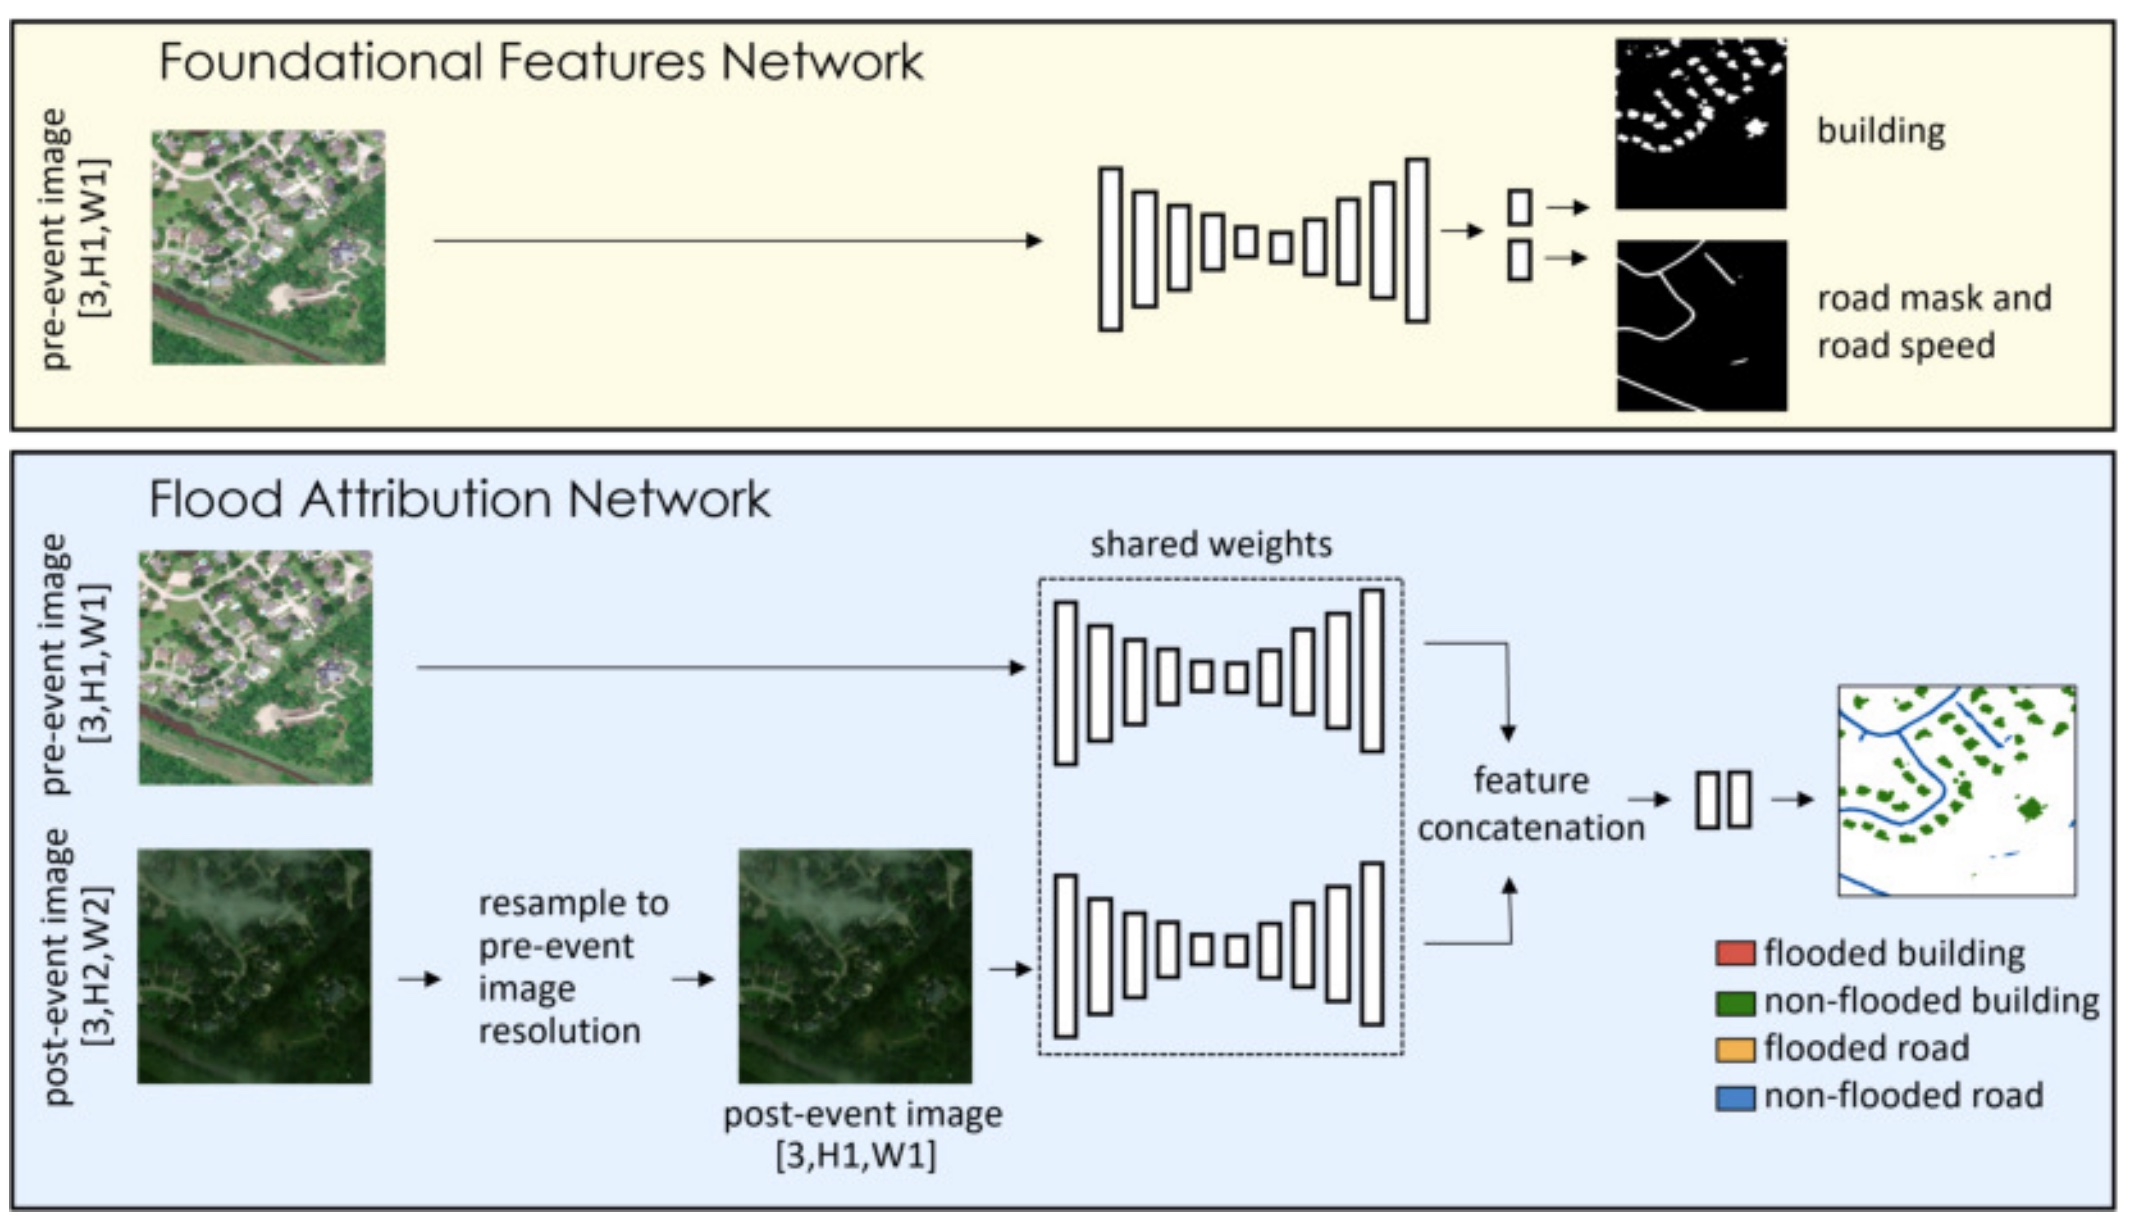
\includegraphics[width=1\linewidth]{figures/baseline.jpg}
   \caption{Schematic of the baseline method. The foundation network is a U-Net style segmentation network with a ResNet34 encoder. The
flood attribution network consists of the same U-Net style segmentation network and ResNet34 encoder, but as siamese networks whereby
a pre-event and post-event image are fed through the network with output features concatenated before the final convolutional layers.}
   \label{fig:baseline}
\end{figure}

\subsubsection{Foundation network}
For the foundation network, the baseline model uses a U-Net \cite{ronneberger2015unet} style segmentation model
with ResNet34 encoder \cite{he2015deep}. The loss is binary cross entropy loss for building segmentation, and a weighted average of Dice loss and Focal loss for road segmentation.

\subsubsection{Flood network}
The Flood network baseline model takes both pre-and post-images in a Siamese convolutional neural network \cite{koch2015siamese} to
generate flood predictions. It was shown that this network is suitable
method for detecting changes in high resolution satellite
imagery \cite{8451652}. This network consists of two identical
branches with shared weights and enables feature extraction
from pre- and post-event image pairs. It uses the same
type of architecture that we use for the foundation features
network. As a Siamese network, one branch receives the
pre-event image as input, while the other branch receives
the post-event image as input. Each branch’s output features
are concatenated, followed by two more convolutional layers
with the last layer producing the 
flood prediction mask.


\subsection{Our method}

Our technical approach is to replace the UNet model and ResNet encoder used by the baseline solution with other CNN and transformer models to see which performs best. To focus on testing our hypothesis about CNN vs transformer architectures, we will reuse the rest of the baseline solution’s source code \cite{spacenet8_baseline} to avoid re-implementing data preprocessing and post-processing logic.

The SpaceNet7 challenge \cite{spacenet7} winners \cite{spacenet7_solutions} provide a source of inspiration of what other CNN model architectures to try. The SpaceNet7 challenge is segmenting buildings from satellite imagery. We expect architectures that performed well on SpaceNet7 to also do well for SpaceNet8 because segmenting buildings is part of both challenges. See \ref{fig:spacenet7}.

\begin{figure}[t]
  \centering
   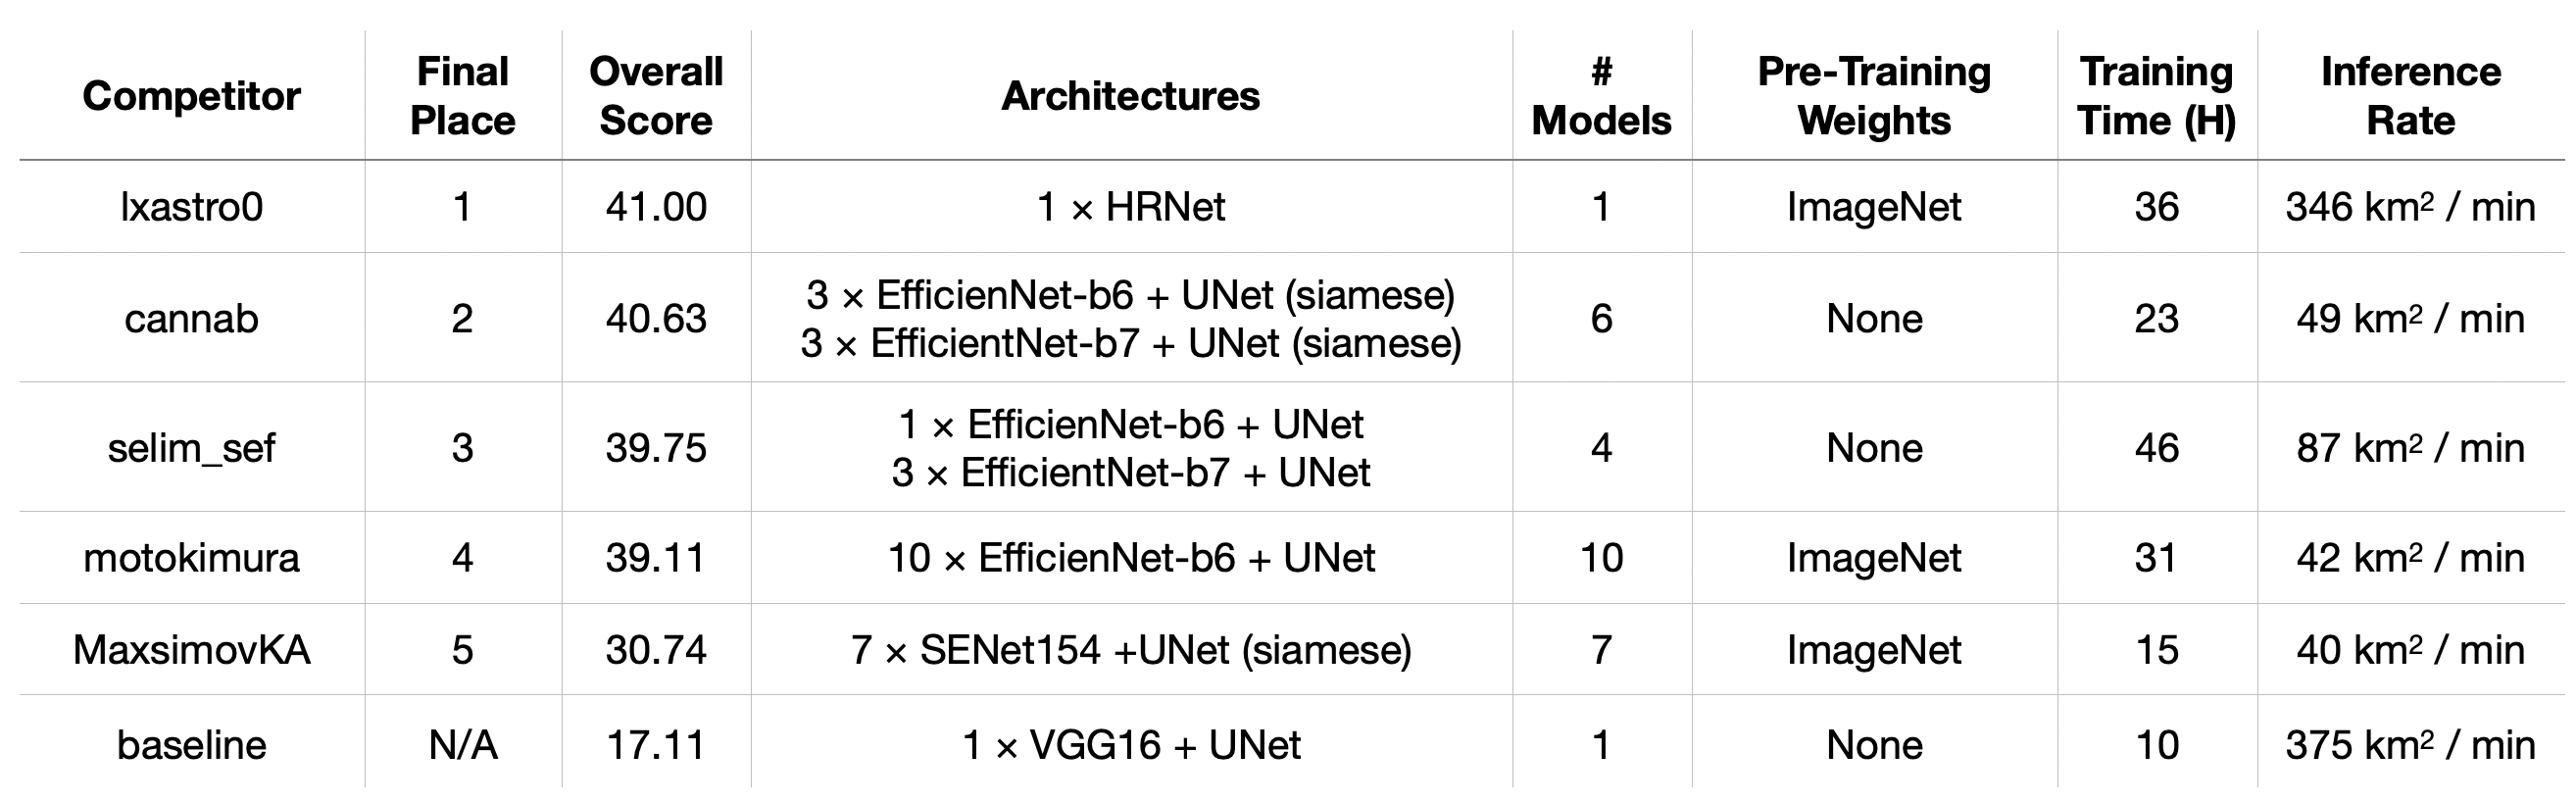
\includegraphics[width=1\linewidth]{figures/spacenet7-winners.png}
   \caption{Architectures used by SpaceNet7 winners}
   \label{fig:spacenet7}
\end{figure}

\subsubsection{Convolutional Architectures}
HRNet is a high-resolution convolutional neural network designed for tasks such as semantic segmentation, object detection, and image classification, while maintaining high-resolution representations throughout the entire process \cite{hrnet}. HRNet starts with a high-resolution convolution stream and gradually adds high-to-low resolution convolution streams one by one. The multi-resolution streams are connected in parallel, allowing repeated multi-resolution fusions by exchanging information across the parallel streams. Figure \ref{fig:HRNet} show the basic architecture of an HRNet. 

\begin{figure}[t]
  \centering
   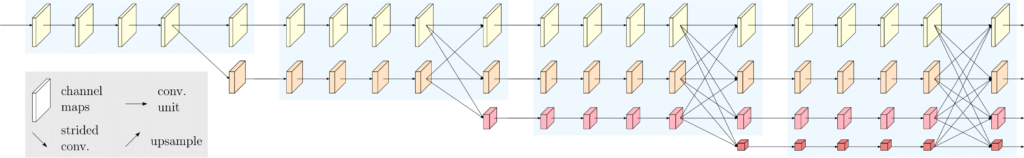
\includegraphics[width=1\linewidth]{figures/HRNet.png}
   \caption{An example of an HRNet. Only the main body is shown.}
   \label{fig:HRNet}
\end{figure}

In the context of this project, we would try to replace the baseline UNet with this more advanced HRNet and fine-tune it based on the two different tasks. In the winning solution of SpaceNet7 \cite{spacenet7_winning}, they leveraged the advantage of HRNet’s ability to maintain high-resolution representations to better capture fine-grain details. We also hope this advantage could help us achieve more precise results, especially by better characterizing obscure objects such as roads obstructed by floodwaters and buildings with water present in their proximity.

\subsubsection{Vision Transformer Architectures}
Dosovitskiy et. al. introduce Vision Transformers (ViT) \cite{dosovitskiy2021image} for image classification tasks. Their approach is to split an image into patches, attach a learned position embedding, feed the patches through a transformer and then use the transformer output for classification with an MLP. They find ViT can beat state-of-the-art CNNs when transferring pre-trained models to smaller datasets. ViT also requires less compute resources to train. While ViT was originally used for object classification, it has since been extended to semantic segmentation tasks.

On semantic segmentation benchmarks, the current best performing models are variants of InternImage, BEiT, and Swin Transformer \cite{paperswithcode_segmentation}. InternImage is based on deformable convolutions \cite{wang2023internimage} while BEiT \cite{bao2022beit} and Swim \cite{liu2021swin} are based on vision transformers.

Our approach is to take pretrained models and fine-tune them to see how well they generalize to the task of flood detection.
For each choice of backbone model we will download a pre-trained model and fine-tune it on the SpaceNet challenge data. We will tune the hyperparameters of each backbone individually, because the choice of hyperparameters for the baseline may not be optimal for the other backbones. We will start by training on a subset of the data for a limited number of epochs to compare initial hyperparameter values and continue training for more epochs on more data for the most promising candidates. To test the secondary hypothesis that an ensemble with both transformer and CNN models will outperform ensembles with only CNNs or only transformers, we will combine predictions from different pairs of the models trained earlier in the project and see which combinations do best.


\section{Preliminary Results}

We trained the baseline model to get a better understanding of the workflow and the dataset. Prior to training, several steps were executed to generate annotation masks from geojson data. We then trained baseline model networks using single P6000 GPU for 30 epoch (8 hours).
A series of post-processing steps are then taken (morphological opening with a structuring element of size 5, mask polygonization, topology preserving polygon simplification with a distance tolerance of 0.75 meters) before a final prediction of flooded vs not-flooded is made. The output of the image  \cite{spacenet8} until a final prediction of is made. We were able to make mask inference (Fig. \ref{fig:predictions}), and in the process of post-processing to obtain final predictions. 

\begin{figure}[t]
  \centering
   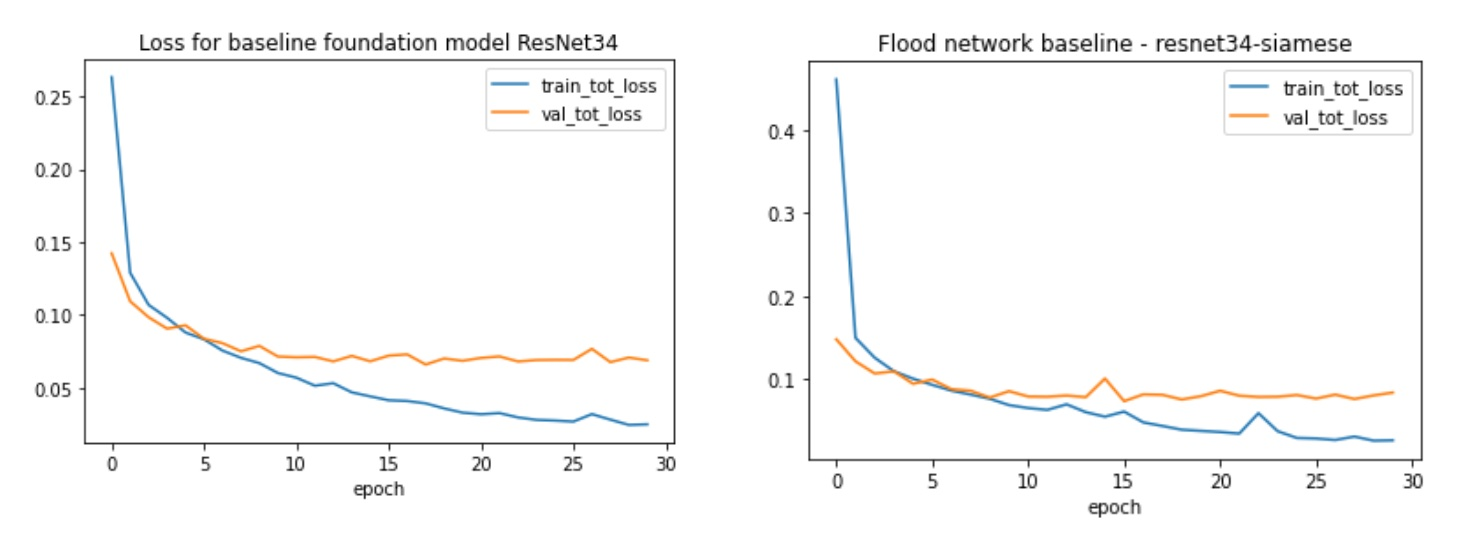
\includegraphics[width=1\linewidth]{figures/loss.jpg}
   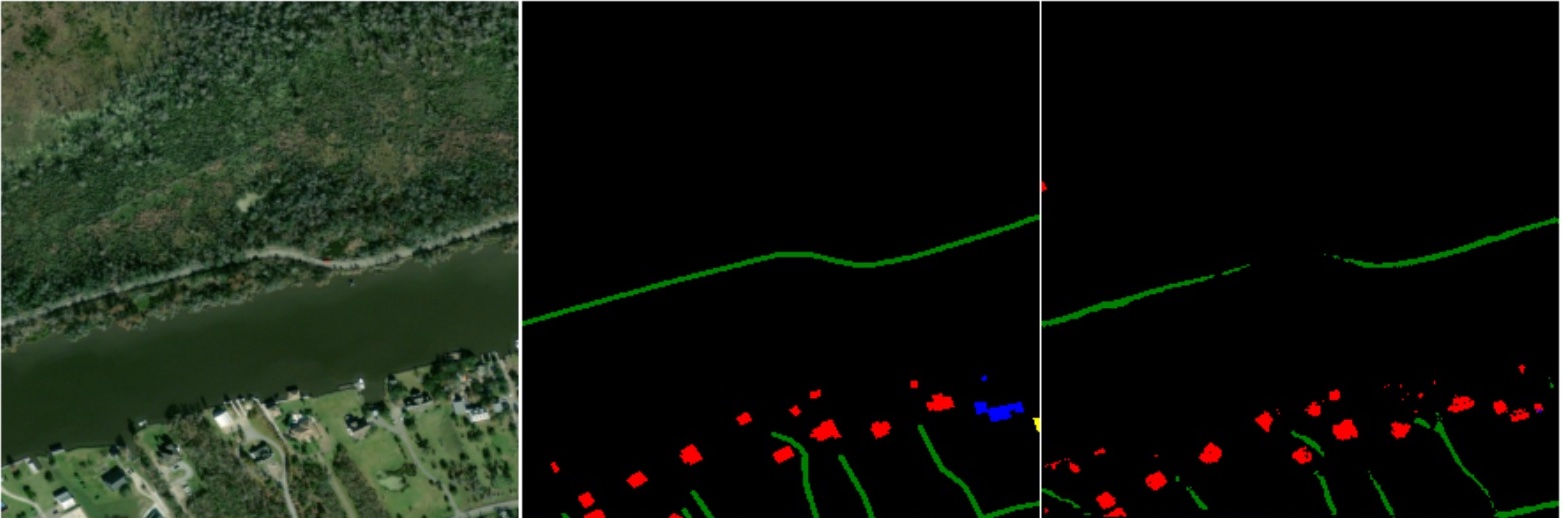
\includegraphics[width=1\linewidth]{figures/baseline_predictions1.jpg}
   \caption{(Up) Loss functions for foundation and flood networks for baseline model. (Below) Example of a raw image, ground truth, prediction (from left to right). Baseline model predicts general building and road shapes.}
   \label{fig:predictions}
\end{figure}
%%%%%%%%% REFERENCES
{\small
\bibliographystyle{ieee_fullname}
\bibliography{egbib}
}

\end{document}
